
%% bare_conf.tex
%% V1.4a
%% 2014/09/17
%% by Michael Shell
%% See:
%% http://www.michaelshell.org/
%% for current contact information.
%%
%% This is a skeleton file demonstrating the use of IEEEtran.cls
%% (requires IEEEtran.cls version 1.8a or later) with an IEEE
%% conference paper.
%%
%% Support sites:
%% http://www.michaelshell.org/tex/ieeetran/
%% http://www.ctan.org/tex-archive/macros/latex/contrib/IEEEtran/
%% and
%% http://www.ieee.org/

%%*************************************************************************
%% Legal Notice:
%% This code is offered as-is without any warranty either expressed or
%% implied; without even the implied warranty of MERCHANTABILITY or
%% FITNESS FOR A PARTICULAR PURPOSE!
%% User assumes all risk.
%% In no event shall IEEE or any contributor to this code be liable for
%% any damages or losses, including, but not limited to, incidental,
%% consequential, or any other damages, resulting from the use or misuse
%% of any information contained here.
%%
%% All comments are the opinions of their respective authors and are not
%% necessarily endorsed by the IEEE.
%%
%% This work is distributed under the LaTeX Project Public License (LPPL)
%% ( http://www.latex-project.org/ ) version 1.3, and may be freely used,
%% distributed and modified. A copy of the LPPL, version 1.3, is included
%% in the base LaTeX documentation of all distributions of LaTeX released
%% 2003/12/01 or later.
%% Retain all contribution notices and credits.
%% ** Modified files should be clearly indicated as such, including  **
%% ** renaming them and changing author support contact information. **
%%
%% File list of work: IEEEtran.cls, IEEEtran_HOWTO.pdf, bare_adv.tex,
%%                    bare_conf.tex, bare_jrnl.tex, bare_conf_compsoc.tex,
%%                    bare_jrnl_compsoc.tex, bare_jrnl_transmag.tex
%%*************************************************************************


% *** Authors should verify (and, if needed, correct) their LaTeX system  ***
% *** with the testflow diagnostic prior to trusting their LaTeX platform ***
% *** with production work. IEEE's font choices and paper sizes can       ***
% *** trigger bugs that do not appear when using other class files.       ***                          ***
% The testflow support page is at:
% http://www.michaelshell.org/tex/testflow/



\documentclass[conference]{IEEEtran}
% Some Computer Society conferences also require the compsoc mode option,
% but others use the standard conference format.
%
% If IEEEtran.cls has not been installed into the LaTeX system files,
% manually specify the path to it like:
% \documentclass[conference]{../sty/IEEEtran}





% Some very useful LaTeX packages include:
% (uncomment the ones you want to load)


% *** MISC UTILITY PACKAGES ***
%
%\usepackage{ifpdf}
% Heiko Oberdiek's ifpdf.sty is very useful if you need conditional
% compilation based on whether the output is pdf or dvi.
% usage:
% \ifpdf
%   % pdf code
% \else
%   % dvi code
% \fi
% The latest version of ifpdf.sty can be obtained from:
% http://www.ctan.org/tex-archive/macros/latex/contrib/oberdiek/
% Also, note that IEEEtran.cls V1.7 and later provides a builtin
% \ifCLASSINFOpdf conditional that works the same way.
% When switching from latex to pdflatex and vice-versa, the compiler may
% have to be run twice to clear warning/error messages.






% *** CITATION PACKAGES ***
%
\usepackage{cite}
% cite.sty was written by Donald Arseneau
% V1.6 and later of IEEEtran pre-defines the format of the cite.sty package
% \cite{} output to follow that of IEEE. Loading the cite package will
% result in citation numbers being automatically sorted and properly
% "compressed/ranged". e.g., [1], [9], [2], [7], [5], [6] without using
% cite.sty will become [1], [2], [5]--[7], [9] using cite.sty. cite.sty's
% \cite will automatically add leading space, if needed. Use cite.sty's
% noadjust option (cite.sty V3.8 and later) if you want to turn this off
% such as if a citation ever needs to be enclosed in parenthesis.
% cite.sty is already installed on most LaTeX systems. Be sure and use
% version 5.0 (2009-03-20) and later if using hyperref.sty.
% The latest version can be obtained at:
% http://www.ctan.org/tex-archive/macros/latex/contrib/cite/
% The documentation is contained in the cite.sty file itself.






% *** GRAPHICS RELATED PACKAGES ***
%

\ifCLASSINFOpdf
  \usepackage[pdftex]{graphicx}
  % declare the path(s) where your graphic files are
  \graphicspath{{fig/}
  % and their extensions so you won't have to specify these with
  % every instance of \includegraphics
  \DeclareGraphicsExtensions{.pdf,.jpeg,.png}
\else
  % or other class option (dvipsone, dvipdf, if not using dvips). graphicx
  % will default to the driver specified in the system graphics.cfg if no
  % driver is specified.
  \usepackage[dvips]{graphicx}
  % declare the path(s) where your graphic files are
  \graphicspath{{fig/}}
  % and their extensions so you won't have to specify these with
  % every instance of \includegraphics
  \DeclareGraphicsExtensions{.eps,.pdf,.jpeg,.png}
\fi
% graphicx was written by David Carlisle and Sebastian Rahtz. It is
% required if you want graphics, photos, etc. graphicx.sty is already
% installed on most LaTeX systems. The latest version and documentation
% can be obtained at:
% http://www.ctan.org/tex-archive/macros/latex/required/graphics/
% Another good source of documentation is "Using Imported Graphics in
% LaTeX2e" by Keith Reckdahl which can be found at:
% http://www.ctan.org/tex-archive/info/epslatex/
%
% latex, and pdflatex in dvi mode, support graphics in encapsulated
% postscript (.eps) format. pdflatex in pdf mode supports graphics
% in .pdf, .jpeg, .png and .mps (metapost) formats. Users should ensure
% that all non-photo figures use a vector format (.eps, .pdf, .mps) and
% not a bitmapped formats (.jpeg, .png). IEEE frowns on bitmapped formats
% which can result in "jaggedy"/blurry rendering of lines and letters as
% well as large increases in file sizes.
%
% You can find documentation about the pdfTeX application at:
% http://www.tug.org/applications/pdftex





% *** MATH PACKAGES ***
%
\usepackage[cmex10]{amsmath}
% A popular package from the American Mathematical Society that provides
% many useful and powerful commands for dealing with mathematics. If using
% it, be sure to load this package with the cmex10 option to ensure that
% only type 1 fonts will utilized at all point sizes. Without this option,
% it is possible that some math symbols, particularly those within
% footnotes, will be rendered in bitmap form which will result in a
% document that can not be IEEE Xplore compliant!
%
% Also, note that the amsmath package sets \interdisplaylinepenalty to 10000
% thus preventing page breaks from occurring within multiline equations. Use:
\interdisplaylinepenalty=2500
% after loading amsmath to restore such page breaks as IEEEtran.cls normally
% does. amsmath.sty is already installed on most LaTeX systems. The latest
% version and documentation can be obtained at:
% http://www.ctan.org/tex-archive/macros/latex/required/amslatex/math/
\usepackage{amsfonts}





% *** SPECIALIZED LIST PACKAGES ***
%
\usepackage{algorithmic}
% algorithmic.sty was written by Peter Williams and Rogerio Brito.
% This package provides an algorithmic environment fo describing algorithms.
% You can use the algorithmic environment in-text or within a figure
% environment to provide for a floating algorithm. Do NOT use the algorithm
% floating environment provided by algorithm.sty (by the same authors) or
% algorithm2e.sty (by Christophe Fiorio) as IEEE does not use dedicated
% algorithm float types and packages that provide these will not provide
% correct IEEE style captions. The latest version and documentation of
% algorithmic.sty can be obtained at:
% http://www.ctan.org/tex-archive/macros/latex/contrib/algorithms/
% There is also a support site at:
% http://algorithms.berlios.de/index.html
% Also of interest may be the (relatively newer and more customizable)
% algorithmicx.sty package by Szasz Janos:
% http://www.ctan.org/tex-archive/macros/latex/contrib/algorithmicx/




% *** ALIGNMENT PACKAGES ***
%
%\usepackage{array}
% Frank Mittelbach's and David Carlisle's array.sty patches and improves
% the standard LaTeX2e array and tabular environments to provide better
% appearance and additional user controls. As the default LaTeX2e table
% generation code is lacking to the point of almost being broken with
% respect to the quality of the end results, all users are strongly
% advised to use an enhanced (at the very least that provided by array.sty)
% set of table tools. array.sty is already installed on most systems. The
% latest version and documentation can be obtained at:
% http://www.ctan.org/tex-archive/macros/latex/required/tools/


% IEEEtran contains the IEEEeqnarray family of commands that can be used to
% generate multiline equations as well as matrices, tables, etc., of high
% quality.




% *** SUBFIGURE PACKAGES ***
\ifCLASSOPTIONcompsoc
 \usepackage[caption=false,font=normalsize,labelfont=sf,textfont=sf]{subfig}
\else
 \usepackage[caption=false,font=footnotesize]{subfig}
\fi
% subfig.sty, written by Steven Douglas Cochran, is the modern replacement
% for subfigure.sty, the latter of which is no longer maintained and is
% incompatible with some LaTeX packages including fixltx2e. However,
% subfig.sty requires and automatically loads Axel Sommerfeldt's caption.sty
% which will override IEEEtran.cls' handling of captions and this will result
% in non-IEEE style figure/table captions. To prevent this problem, be sure
% and invoke subfig.sty's "caption=false" package option (available since
% subfig.sty version 1.3, 2005/06/28) as this is will preserve IEEEtran.cls
% handling of captions.
% Note that the Computer Society format requires a larger sans serif font
% than the serif footnote size font used in traditional IEEE formatting
% and thus the need to invoke different subfig.sty package options depending
% on whether compsoc mode has been enabled.
%
% The latest version and documentation of subfig.sty can be obtained at:
% http://www.ctan.org/tex-archive/macros/latex/contrib/subfig/




% *** FLOAT PACKAGES ***
%
%\usepackage{fixltx2e}
% fixltx2e, the successor to the earlier fix2col.sty, was written by
% Frank Mittelbach and David Carlisle. This package corrects a few problems
% in the LaTeX2e kernel, the most notable of which is that in current
% LaTeX2e releases, the ordering of single and double column floats is not
% guaranteed to be preserved. Thus, an unpatched LaTeX2e can allow a
% single column figure to be placed prior to an earlier double column
% figure. The latest version and documentation can be found at:
% http://www.ctan.org/tex-archive/macros/latex/base/


\usepackage{stfloats}
% stfloats.sty was written by Sigitas Tolusis. This package gives LaTeX2e
% the ability to do double column floats at the bottom of the page as well
% as the top. (e.g., "\begin{figure*}[!b]" is not normally possible in
% LaTeX2e). It also provides a command:
\fnbelowfloat
% to enable the placement of footnotes below bottom floats (the standard
% LaTeX2e kernel puts them above bottom floats). This is an invasive package
% which rewrites many portions of the LaTeX2e float routines. It may not work
% with other packages that modify the LaTeX2e float routines. The latest
% version and documentation can be obtained at:
% http://www.ctan.org/tex-archive/macros/latex/contrib/sttools/
% Do not use the stfloats baselinefloat ability as IEEE does not allow
% \baselineskip to stretch. Authors submitting work to the IEEE should note
% that IEEE rarely uses double column equations and that authors should try
% to avoid such use. Do not be tempted to use the cuted.sty or midfloat.sty
% packages (also by Sigitas Tolusis) as IEEE does not format its papers in
% such ways.
% Do not attempt to use stfloats with fixltx2e as they are incompatible.
% Instead, use Morten Hogholm'a dblfloatfix which combines the features
% of both fixltx2e and stfloats:
%
% \usepackage{dblfloatfix}
% The latest version can be found at:
% http://www.ctan.org/tex-archive/macros/latex/contrib/dblfloatfix/




% *** PDF, URL AND HYPERLINK PACKAGES ***
%
\usepackage{url}
% url.sty was written by Donald Arseneau. It provides better support for
% handling and breaking URLs. url.sty is already installed on most LaTeX
% systems. The latest version and documentation can be obtained at:
% http://www.ctan.org/tex-archive/macros/latex/contrib/url/
% Basically, \url{my_url_here}.




% *** Do not adjust lengths that control margins, column widths, etc. ***
% *** Do not use packages that alter fonts (such as pslatex).         ***
% There should be no need to do such things with IEEEtran.cls V1.6 and later.
% (Unless specifically asked to do so by the journal or conference you plan
% to submit to, of course. )


% correct bad hyphenation here
\hyphenation{op-tical net-works semi-conduc-tor}

\renewcommand\IEEEkeywordsname{Keywords}

\begin{document}
%
% paper title
% Titles are generally capitalized except for words such as a, an, and, as,
% at, but, by, for, in, nor, of, on, or, the, to and up, which are usually
% not capitalized unless they are the first or last word of the title.
% Linebreaks \\ can be used within to get better formatting as desired.
% Do not put math or special symbols in the title.
\title{A New Dynamically Reference Point Adaptation Mechanism in indicator-based EMOA
based on weak convergence detection}

% author names and affiliations
% use a multiple column layout for up to three different
% affiliations
\author{
  \IEEEauthorblockN{Weiduo Liao}
  \IEEEauthorblockA{School of Electrical and\\Computer Engineering\\
  Georgia Institute of Technology\\
  Atlanta, Georgia 30332--0250\\
  Email: \url{http://www.michaelshell.org/contact.html}}
  \and
  \IEEEauthorblockN{sssss}
  \IEEEauthorblockA{Twentieth Century Fox\\
  Springfield, USA\\
  Email: homer@thesimpsons.com}
  \and
  \IEEEauthorblockN{ssss}
  \IEEEauthorblockA{Starfleet Academy\\
  San Francisco, California 96678--2391\\
  Telephone: (800) 555--1212\\
  Fax: (888) 555--1212}
}

% conference papers do not typically use \thanks and this command
% is locked out in conference mode. If really needed, such as for
% the acknowledgment of grants, issue a \IEEEoverridecommandlockouts
% after \documentclass

% for over three affiliations, or if they all won't fit within the width
% of the page, use this alternative format:
%
%\author{\IEEEauthorblockN{Michael Shell\IEEEauthorrefmark{1},
%Homer Simpson\IEEEauthorrefmark{2},
%James Kirk\IEEEauthorrefmark{3},
%Montgomery Scott\IEEEauthorrefmark{3} and
%Eldon Tyrell\IEEEauthorrefmark{4}}
%\IEEEauthorblockA{\IEEEauthorrefmark{1}\\
%School of Electrical and Computer Engineering\\
%Georgia Institute of Technology,
%Atlanta, Georgia 30332--0250\\ 
%Email: see http://www.michaelshell.org/contact.html}
%\IEEEauthorblockA{\IEEEauthorrefmark{2}Twentieth Century Fox, Springfield, USA\\
%Email: homer@thesimpsons.com}
%\IEEEauthorblockA{\IEEEauthorrefmark{3}Starfleet Academy, San Francisco,\\
%California 96678-2391\\
%Telephone: (800) 555--1212, Fax: (888) 555--1212}
%\IEEEauthorblockA{\IEEEauthorrefmark{4}Tyrell Inc., 123 Replicant Street,\\
%Los Angeles, California 90210--4321}}




% use for special paper notices
%\IEEEspecialpapernotice{(Invited Paper)}




% make the title area
\maketitle

% As a general rule, do not put math, special symbols or citations
% in the abstract
\begin{abstract}
The abstract goes here.
\end{abstract}

\begin{IEEEkeywords}
keyword 1; keyword 2
\end{IEEEkeywords}


% For peer review papers, you can put extra information on the cover
% page as needed:
% \ifCLASSOPTIONpeerreview
% \begin{center} \bfseries EDICS Category: 3-BBND \end{center}
% \fi
%
% For peerreview papers, this IEEEtran command inserts a page break and
% creates the second title. It will be ignored for other modes.
\IEEEpeerreviewmaketitle



\section{Introduction}
% no \IEEEPARstart
This demo file is intended to serve as a ``starter file''
for IEEE conference papers produced under \LaTeX\ using
IEEEtran.cls version 1.8a and later.
% You must have at least 2 lines in the paragraph with the drop letter
% (should never be an issue)
I wish you the best of success.

\hfill mds

\hfill September 17, 2014


\subsection{Subsection Heading Here}
Subsection text here.


\subsubsection{Subsubsection Heading Here}
Subsubsection text here.


% An example of a floating figure using the graphicx package.
% Note that \label must occur AFTER (or within) \caption.
% For figures, \caption should occur after the \includegraphics.
% Note that IEEEtran v1.7 and later has special internal code that
% is designed to preserve the operation of \label within \caption
% even when the captionsoff option is in effect. However, because
% of issues like this, it may be the safest practice to put all your
% \label just after \caption rather than within \caption{}.
%
% Reminder: the "draftcls" or "draftclsnofoot", not "draft", class
% option should be used if it is desired that the figures are to be
% displayed while in draft mode.
%
%\begin{figure}[!t]
%\centering
%\includegraphics[width=2.5in]{myfigure}
% where an .eps filename suffix will be assumed under latex,
% and a .pdf suffix will be assumed for pdflatex; or what has been declared
% via \DeclareGraphicsExtensions.
%\caption{Simulation results for the network.}
%\label{fig_sim}
%\end{figure}

% Note that IEEE typically puts floats only at the top, even when this
% results in a large percentage of a column being occupied by floats.


% An example of a double column floating figure using two subfigures.
% (The subfig.sty package must be loaded for this to work.)
% The subfigure \label commands are set within each subfloat command,
% and the \label for the overall figure must come after \caption.
% \hfil is used as a separator to get equal spacing.
% Watch out that the combined width of all the subfigures on a
% line do not exceed the text width or a line break will occur.
%
%\begin{figure*}[!t]
%\centering
%\subfloat[Case I]{\includegraphics[width=2.5in]{box}%
%\label{fig_first_case}}
%\hfil
%\subfloat[Case II]{\includegraphics[width=2.5in]{box}%
%\label{fig_second_case}}
%\caption{Simulation results for the network.}
%\label{fig_sim}
%\end{figure*}
%
% Note that often IEEE papers with subfigures do not employ subfigure
% captions (using the optional argument to \subfloat[]), but instead will
% reference/describe all of them (a), (b), etc., within the main caption.
% Be aware that for subfig.sty to generate the (a), (b), etc., subfigure
% labels, the optional argument to \subfloat must be present. If a
% subcaption is not desired, just leave its contents blank,
% e.g., \subfloat[].


% An example of a floating table. Note that, for IEEE style tables, the
% \caption command should come BEFORE the table and, given that table
% captions serve much like titles, are usually capitalized except for words
% such as a, an, and, as, at, but, by, for, in, nor, of, on, or, the, to
% and up, which are usually not capitalized unless they are the first or
% last word of the caption. Table text will default to \footnotesize as
% IEEE normally uses this smaller font for tables.
% The \label must come after \caption as always.
%
%\begin{table}[!t]
%% increase table row spacing, adjust to taste
%\renewcommand{\arraystretch}{1.3}
% if using array.sty, it might be a good idea to tweak the value of
% \extrarowheight as needed to properly center the text within the cells
%\caption{An Example of a Table}
%\label{table_example}
%\centering
%% Some packages, such as MDW tools, offer better commands for making tables
%% than the plain LaTeX2e tabular which is used here.
%\begin{tabular}{|c||c|}
%\hline
%One & Two\\
%\hline
%Three & Four\\
%\hline
%\end{tabular}
%\end{table}


% Note that the IEEE does not put floats in the very first column
% - or typically anywhere on the first page for that matter. Also,
% in-text middle ("here") positioning is typically not used, but it
% is allowed and encouraged for Computer Society conferences (but
% not Computer Society journals). Most IEEE journals/conferences use
% top floats exclusively.
% Note that, LaTeX2e, unlike IEEE journals/conferences, places
% footnotes above bottom floats. This can be corrected via the
% \fnbelowfloat command of the stfloats package.

% -------------------------------------- main part ---------------------------------------
% 背景介绍:
% 在indicator based 算法里,HV作为唯一的compliant indicator被广泛使用
% SMSEMOA是最简单的一种indicator based 算法   μ+1机制
% FVEMOA是SMSEMOA的一种优化 速度更快 用了 μ+m机制
% reference point要slightly larger then 1+1/H at beginning then decrease to 1+1/H,  
% hisao的paper with linearly decrease mechanism: 
% [1] H. Ishibuchi, R. Imada, N. Masuyama and Y. Nojima. 
% Dynamic Specification of a Reference Point for Hypervolume Calculation in SMS-EMOA[J].
% Proc. of 2018 IEEE Congress on Evolutionary Computation (IEEE CEC 2018)
% 介绍我的 new mechanism:weak convergence detection decrease
% 一篇paper介绍一种robust and efficient的convergence detection criterion
% Introducing a Robust and Efficient Stopping Criterion for MOEAs
% 但是对象是针对indicator的,而我们的算法运行中计算的indicator 
% 每一代的evaluation不一样,没有可比性
% 补充一张记录每次evaluation时以当时estimated的reference point为based 的hv值的图,
% 表示没有可比性(用FVEMOA的)
% 于是我想到了用nadir point的mean来当indicator,表示是否接近pareto front
% 实验图 mean of ln(nadir point)和它的bsf 与hv的变化曲线基本一致
%(hv斜率变0的时候 这个新indicator的斜率也差不多变成0)
% 介绍一个windows 和 windows内的简单线性回归。 
% 因为会有恶化和停滞现象 所以window size要设置的大一点,
% 经过实验用4000次evaluation作为window size不错
% 然后画b的图,给出经过实验 threshold选10^-5不错。

% 实验
% 4种problems要一句话介绍

% -------------------------------- reference point adaptation ------------------------------
% reference point不应该只在刚开始设置而后面都不变,这样如果问题的feasible region很大的时候,初始设置的
% reference point就会离PF很远(画图一个很大的feasible region和PF和reference point)
% 这样的话 在某些问题(倒三角)最后分布在PF上的解 边缘上的解分布很密集【hisao paper】【倒三角图,r很大】
% 因此 necessity of reference point adaptation during the progress of algorithm
%
% 在很多算法中 include SMSEMOA
% The reference point is specified by the following common-use role:
% estimated reference point = r × estimated nadir point, r = 1.1, 
% the estimated nadir point is the vector consists of every maximization objective values of all
% solutions in current population.【图】
%
\section{Reference Point Adaptation}
When hypervolume(HV) is used in indicator-based algorithms, 
one important thing to be considered is that how to specified the reference point.
Before calculating the HV values, reference point needs to be chosen in advance.
However, it is not suggested that the reference point is set only once at the beginning.
\cite{ut}  % undergraduated thesis
This may cause a very far away reference point from solutions
for those problems with a very large feasible space(As shown in Fig. \ref{rpa1}),
as the solutions set is gradually converging to the pareto front
during the iteration of the algorithm process.

\begin{figure}[!t]
  \centering
  \subfloat[The initial generation.]{\label{rpa1:a}
    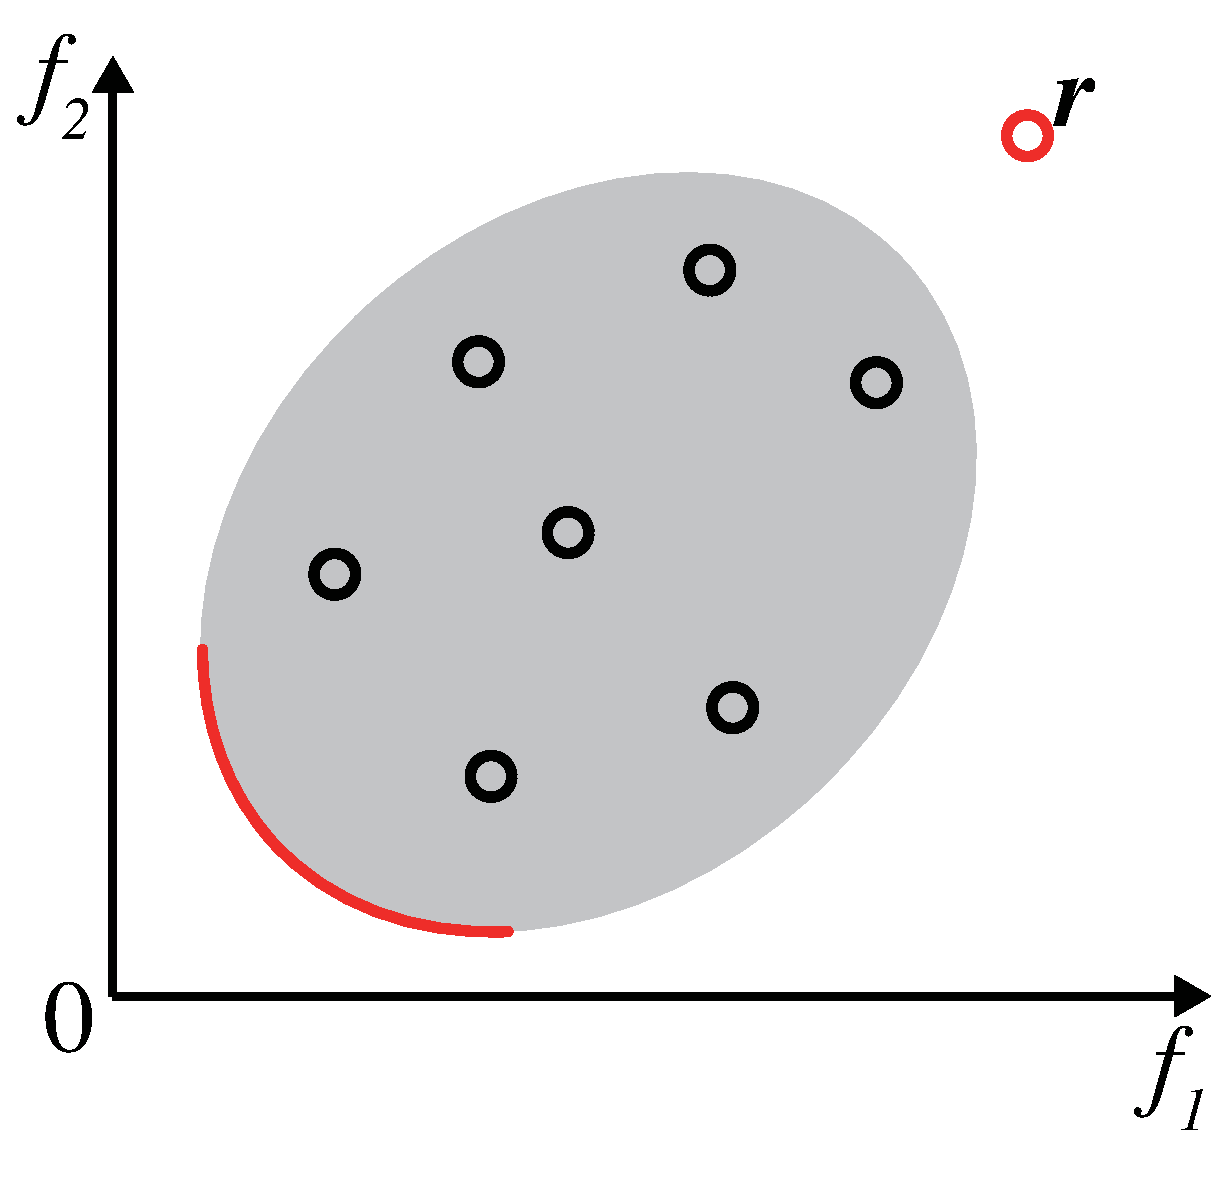
\includegraphics[width=1.5in]{rpa1_1}}\quad
  \subfloat[The final generation.]{\label{rpa1:b}
  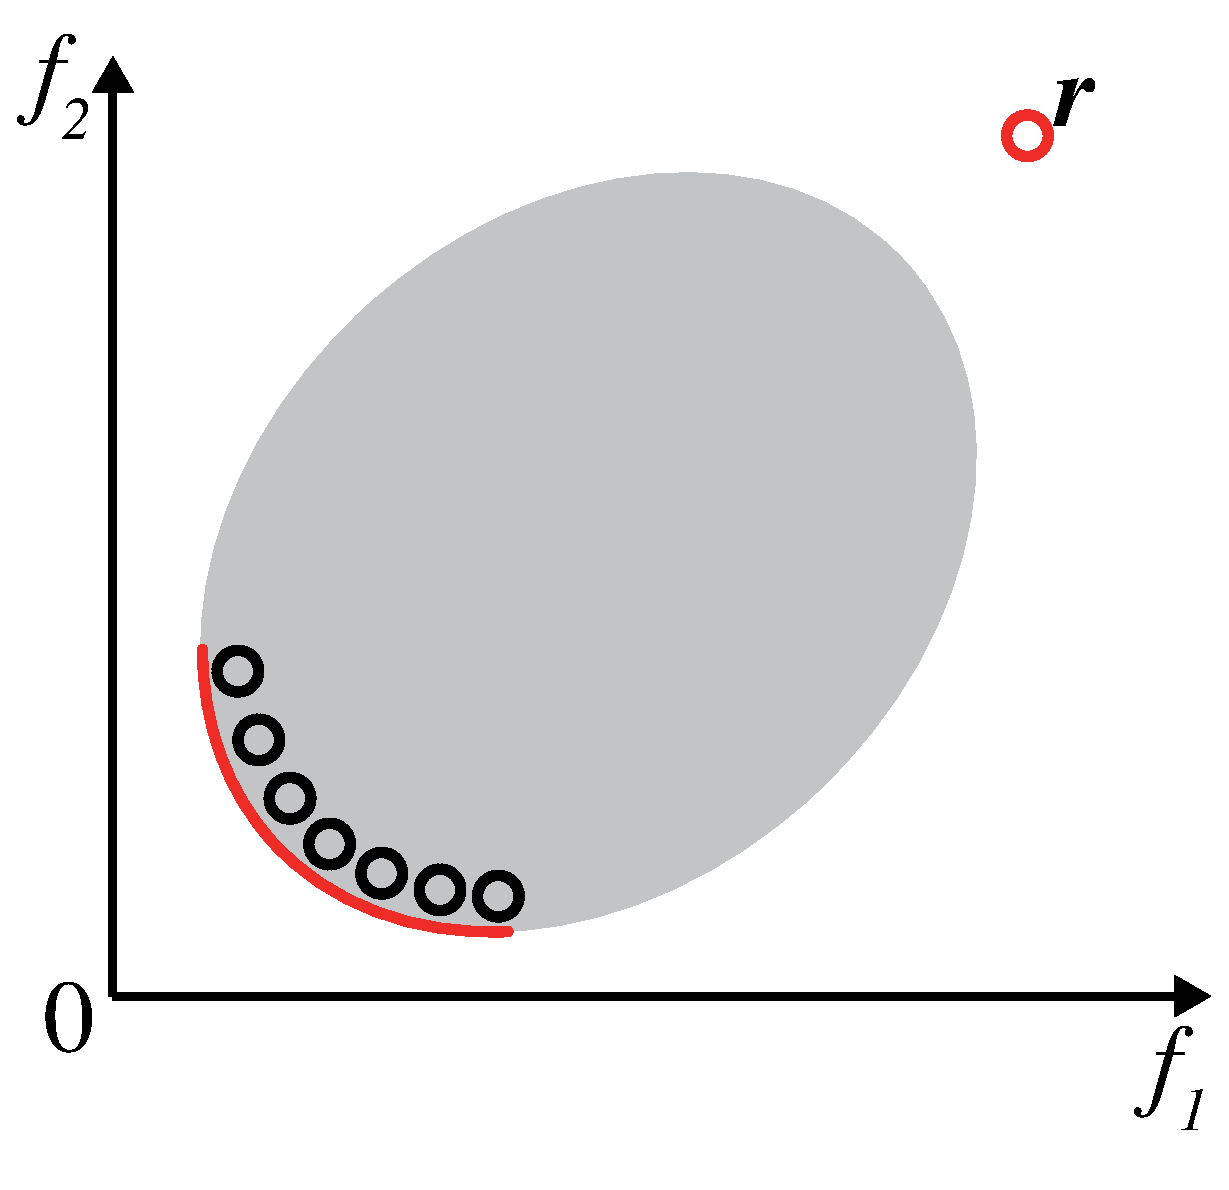
\includegraphics[width=1.5in]{rpa1_2}}\\
  \caption{The reference point is set with a large feasible space.
  pareto front can be far away from reference point.
  The gray region shows the feasible region and the red arc is the corresponding pareto front.
  The red circle $r$ is the reference point calculated by the initial solutions in (\ref{rpa1:a})
  which is randomly generated.
  After some generations, the current solutions reach to the five black circles in (\ref{rpa1:b}), 
  which is far away from the reference point.}
  \label{rpa1}
\end{figure}

There is a big problem when applying this strategy to some problems with specific pareto front shape, 
for example, the inverted-DTLZ1 problem with a inverted-triangular pareto front in 3 dimensions,
that many solutions in the final solutions set will distribute at the boundary of the pareto front
(Fig. \ref{rpa2:a} comparing with Fig. \ref{rpa2:b})\cite{hisao1,hisao2}. 
% Dynamic Specification of a Reference Point for Hypervolume Calculation in SMS-EMOA
% Reference point specification in hypervolume calculation for fair comparison and efficient search
Although it has no effect on the distributions of solutions set 
in problems with triangular pareto front in 3 dimensions 
(Fig. \ref{rpa2:c} comparing with Fig. \ref{rpa2:d}), 
it is necessary using reference point adaptation during the algorithm progress.
And the reason is illustrated detailedly in hisao \cite{hisaos}. % hisao介绍原因的paper。

In many algorithms including SMS-EMOA\cite{smsemoa}, 
the reference point is adapted based on the following rules:
\begin{equation}\label{frpa1}
  RP = r * ENP, r = 1.1.
\end{equation}
Note that the estimated nadir point($ENP$) is the nadir point in current population.
When the solutions in the current population is obtained, 
we use hypervolume as indicator to evaluate the performance of the solutions set. 
Then the reference point used to calculate the hypervolume is calculated by the formula above.
%可以加一个介绍nadir point的图,如果8页不够的话。

\begin{figure}[!t]
  \centering
  \subfloat[The inverted-DTLZ1 problem with a fixed reference point.]{\label{rpa2:a}
    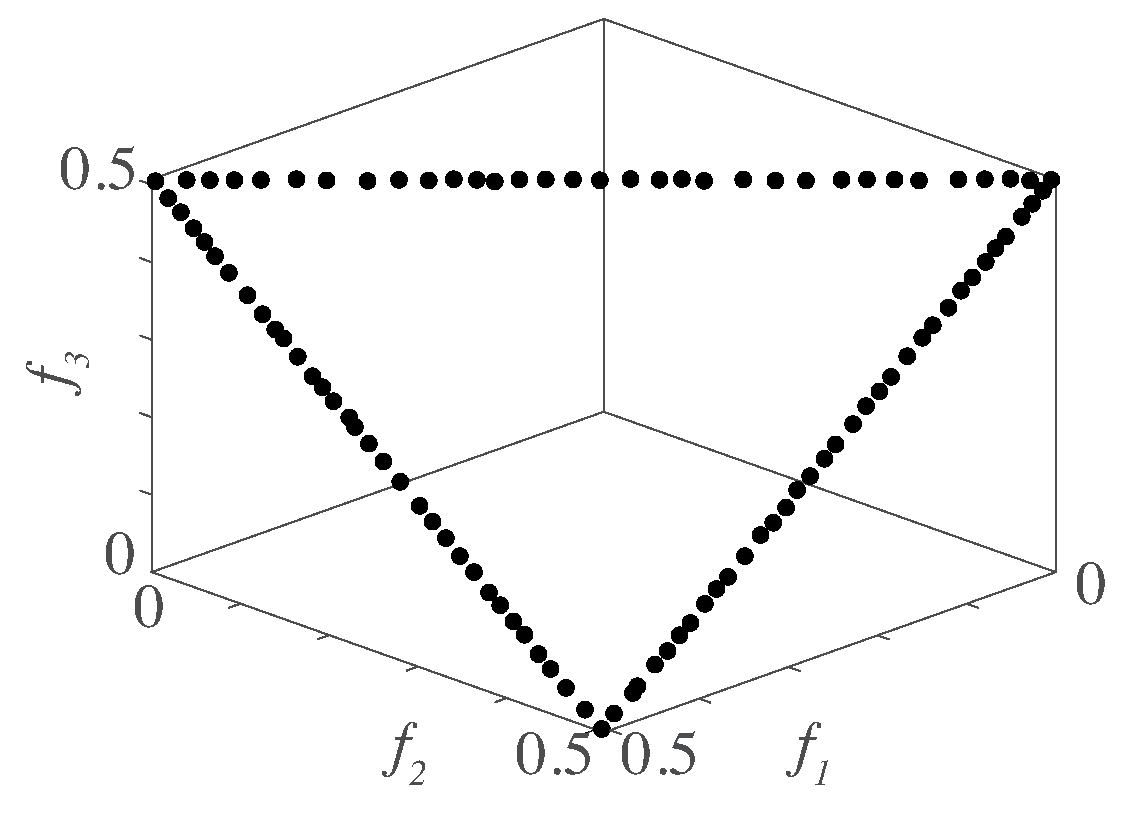
\includegraphics[width=1.5in]{FVEMOA_fixrp_IDTLZ1_evaluation20000_r1__1}}\quad
  \subfloat[The inverted-DTLZ1 problem with a adapted reference point.]{\label{rpa2:b}
    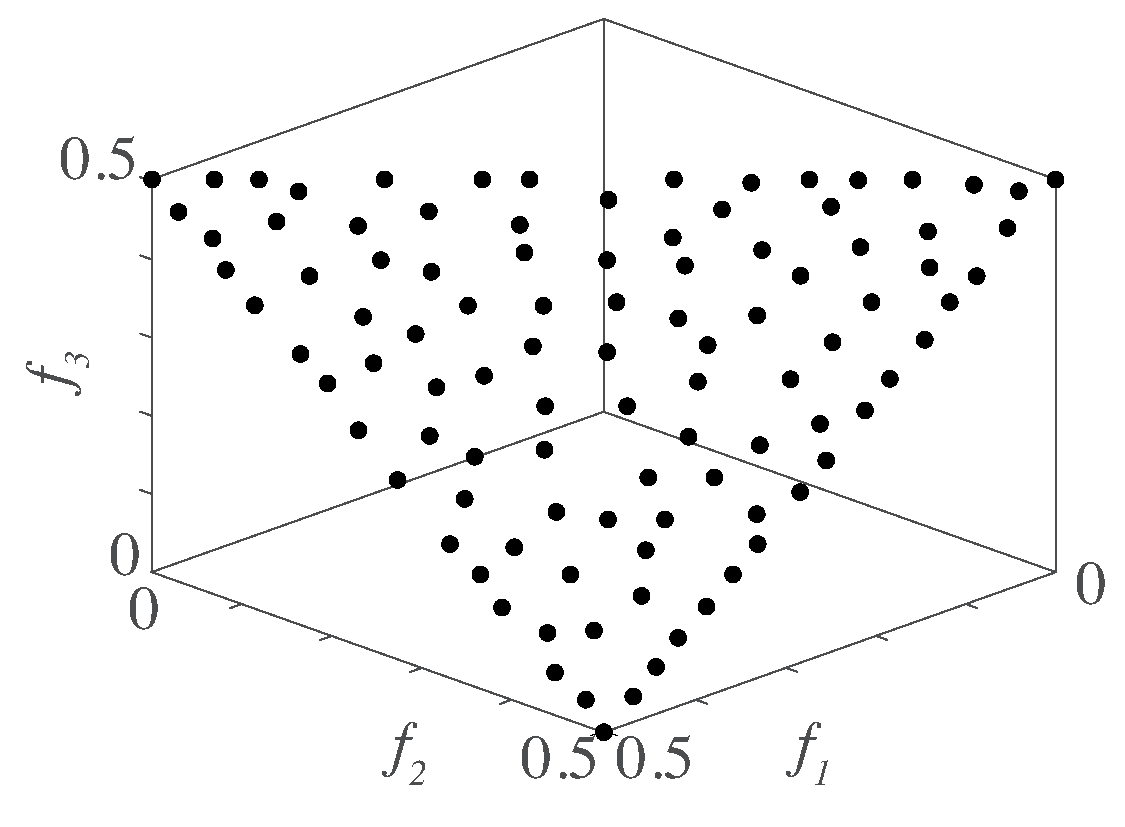
\includegraphics[width=1.5in]{FVEMOA_IDTLZ1_evaluation20000_r1__1}}\\
  \subfloat[The DTLZ1 problem with a fixed reference point.]{\label{rpa2:c}
    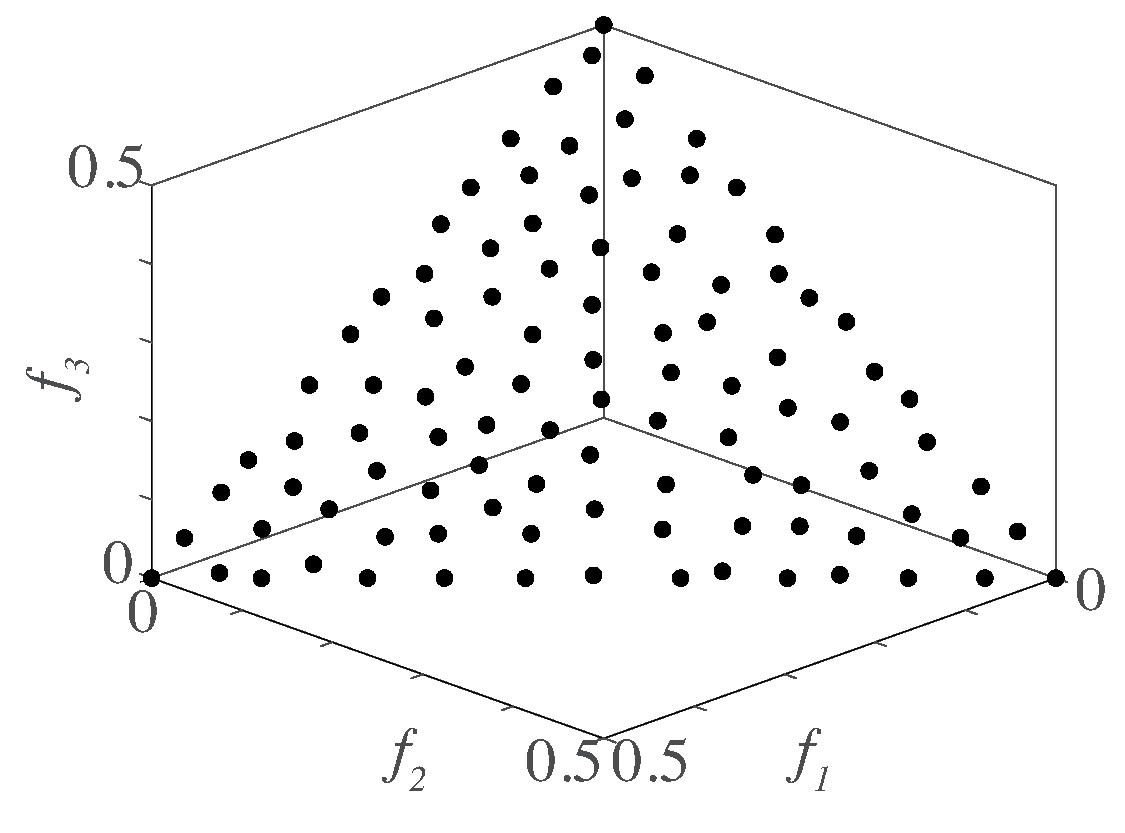
\includegraphics[width=1.5in]{FVEMOA_fixrp_DTLZ1_evaluation20000_r1__1}}\quad
  \subfloat[The DTLZ1 problem with a adapted reference point.]{\label{rpa2:d}
    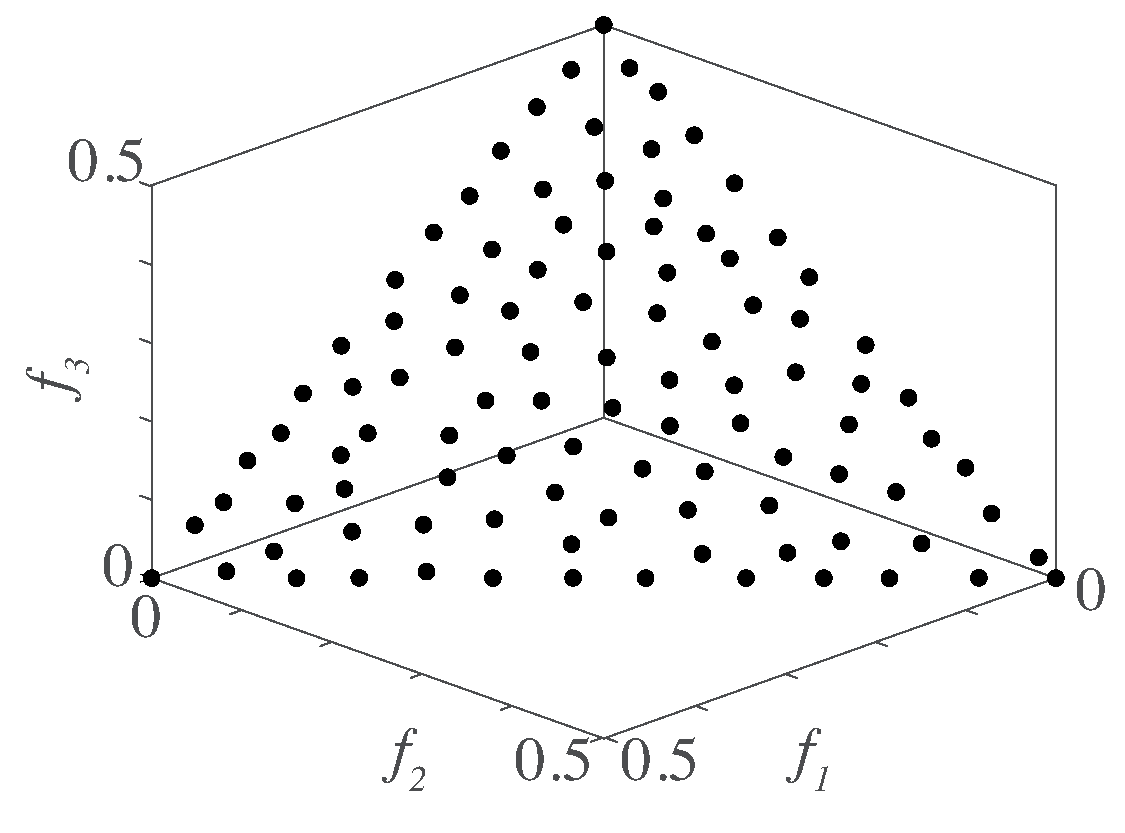
\includegraphics[width=1.5in]{FVEMOA_DTLZ1_evaluation20000_r1__1}}\\
  \caption{The final distribution of solutions set in the inverted-DTLZ1(\ref{rpa2:a} and \ref{rpa2:b}) 
  and the DTLZ1 problem(\ref{rpa2:c} and \ref{rpa2:d}).
  The algorithm is FV-EMOA with population size $= 100$, evaluation number $= 20000$ and $r=1.1$. 
  (\ref{rpa2:a} and \ref{rpa2:c}): the reference point is calculated only once at the initial step;
  (\ref{rpa2:b} and \ref{rpa2:d}): the reference point is adapted based on the formula (\ref{frpa1}).
  All the solutions in the final distribution are at the boundary of the pareto front in (\ref{rpa2:a}),
  which shows the bad effect of a far away reference point
  on the final distribution of inverted-triangular problems.
  This bad effect can not be observed on triangular problems in (\ref{rpa2:c}).
  }
  \label{rpa2}
\end{figure}

% ----------------------------------- dynamic mechanism ------------------------------------
% 在算法运行的不同时期 early stage;final stage, 为了不同的目的,
% (early stage是convergence, final stage是diversity) r应该设置成不同的值【我的本科毕设和hisao】
% 即 r value 应该是随着算法的进行dynamically设置成不同的值。 
%
% unfortunately 对r的研究太少了, 因为在 benchmark问题上, 特别是正三角 r对PF上的解的影响很小
% 但是实际上 在一些问题上 最后PF上解的分布情况是对r很敏感的【hisao paper里的倒三角和最近点问题】
% 
\section{Dynamic Mechanism}
Basically the process of Evolutionary Multi-objective Optimization Algorithm can be separate into
two stages:
\subsubsection{Early Stage} In this stage, 
all the solutions are far away from pareto front.
The main task is to converge the solutions to pareto front.
We also call this stage convergence stage.
\subsubsection{Final Stage} In this stage,
all the solutions are in or near the pareto front.
So the main task is to make the distribution of solutions more evenly in the pareto front.
We also call this stage diversity stage.

For different purposes in these two stages, the $r$ should be treated differently\cite{ut}. 
Not only the reference point but also the value of $r$ 
needs to be adapted in each iteration of algorithm. 
This is called dynamically reference point adaptation. 

Unfortunately, the research on how to specified $r$ is limited.
Only a few papers\cite{hisao1, hisao2, hisao3, zhangqingfuHypE} 
did some research on the reference point. 
% 这方面的研究有限,研究的不够深入
The reason is that, the effect of the location of the reference point on the pareto front 
is not fatal on some benchmark problems, especially triangular pareto front. 
But in fact, on some specific problems, the distribution of solutions on pareto front
strongly depends on the location of the reference point. 
The sensitivity about value of $r$ for solutions is also observerd on some real world problems,
for example, distance minimization problems.
This observation Potential shows the usefulness of the dynamically reference point adaptation
\cite{hisao}.

In this section, we will specify the suggested $r$ values seperately
in the early and final stages.

% ------------------sub-------------- dynamic mechanism ----------------------------------
% --------------- reference point specification for optimal distribution ----------------
% 在hisao的paper中指出r = 1+1/H 在一些问题中(平的PF问题)是最优的设置(画出二维三维图for example),
% 提一句 本文主要的研究问题就是平的PF问题
% 即在算法的最后final stage,所有solution都在PF上,r应该设置成1+1/H。
%
\subsection{Reference Point Specification for Optimal Distribution}
In the final stages, the major purpose is to augment the diversity of solutions set.
More specifically, for inverted-triangular problems, 
the interval between two boundary solutions should be same as that between two inner solutions.
In hisao\cite{hisao}.% 在hisao的paper里,
\begin{equation}\label{e1}
  r=1+\frac{1}{H},
\end{equation}
is the optimal setting for flat(not concave or convex) pareto front problem
(As shown in Fig. \ref{dm1}). $H$ is the number of solutions intervals in 2-dimension 
and the number of interval at each boundary of pareto front in many-dimension.
In Fig. \ref{dm1:a}, $r=1.2(H=5)$ is the optimal setting for a $21$ individuals 
inverted-DTLZ1 problem and a evenly distribution is observed. 
In Fig. \ref{dm1:b} - Fig. \ref{dm1:d}, the inner solutions are decreased and move to
the boundary of pareto front. 

\begin{figure}[!t]
  \centering
  \subfloat[$r=1.2$(optimal).]{\label{dm1:a}
    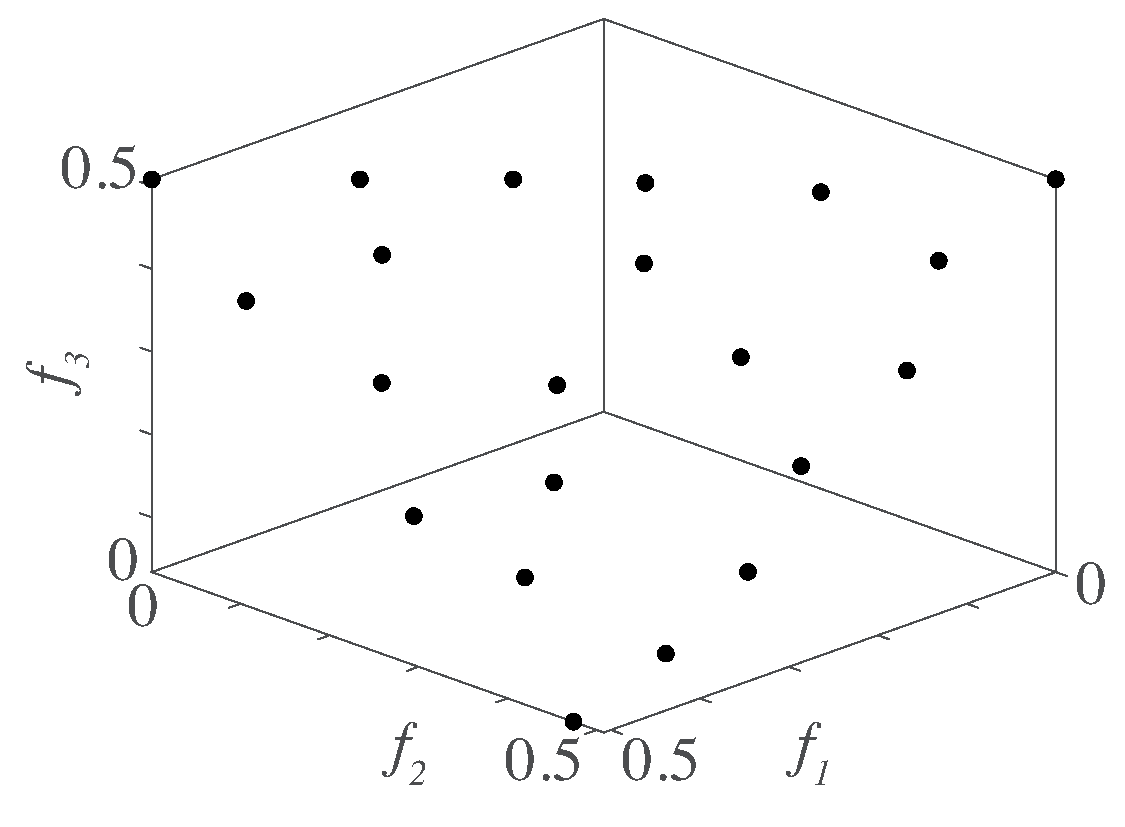
\includegraphics[width=1.5in]{FVEMOA_IDTLZ1_evaluation10000_r1__2_N21}}\quad
  \subfloat[$r=1.5.$]{\label{dm1:b}
    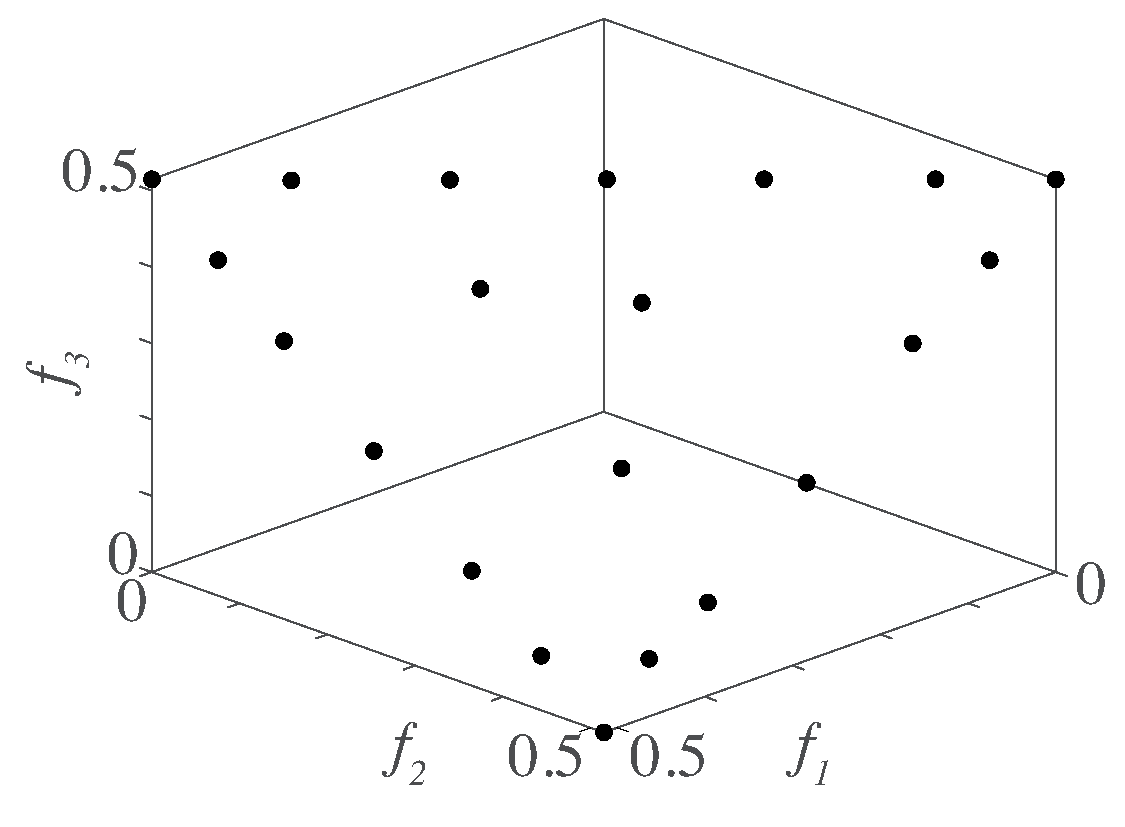
\includegraphics[width=1.5in]{FVEMOA_IDTLZ1_evaluation10000_r1__5_N21}}\\
  \subfloat[$r=2.$]{\label{dm1:c}
    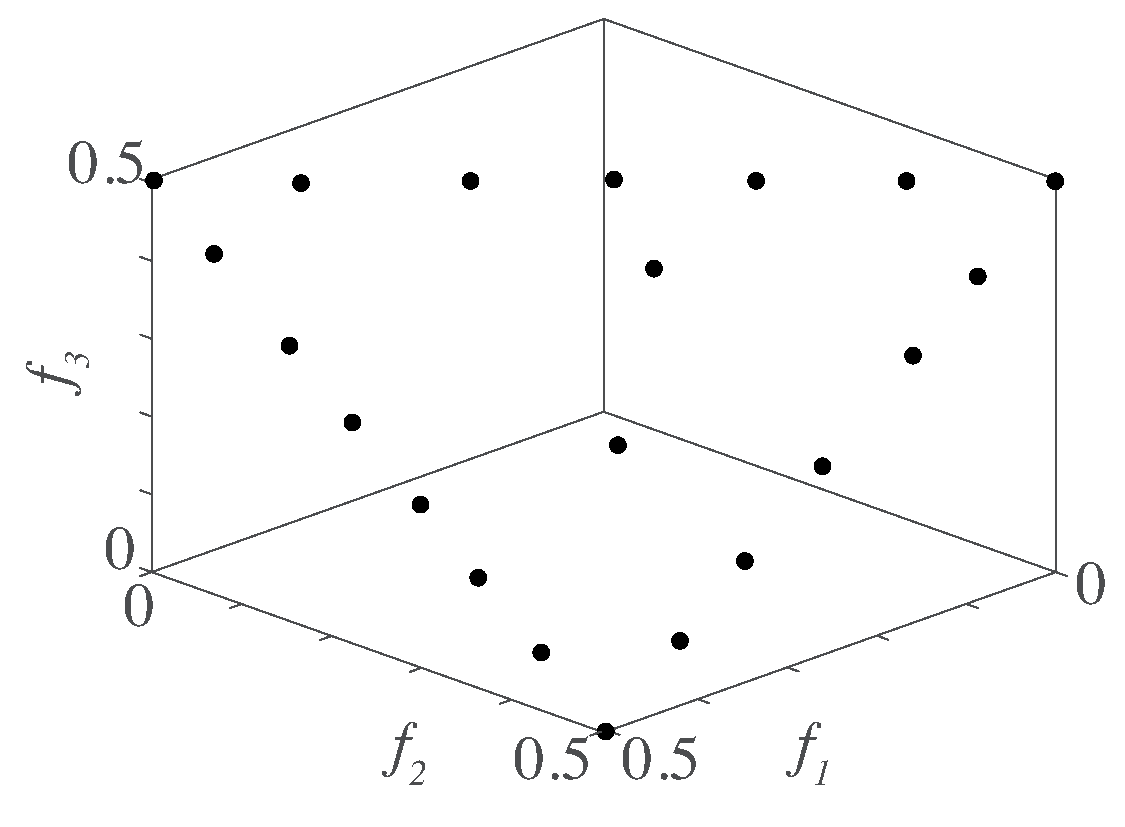
\includegraphics[width=1.5in]{FVEMOA_IDTLZ1_evaluation10000_r2_N21}}\quad
  \subfloat[$r=5.$]{\label{dm1:d}
    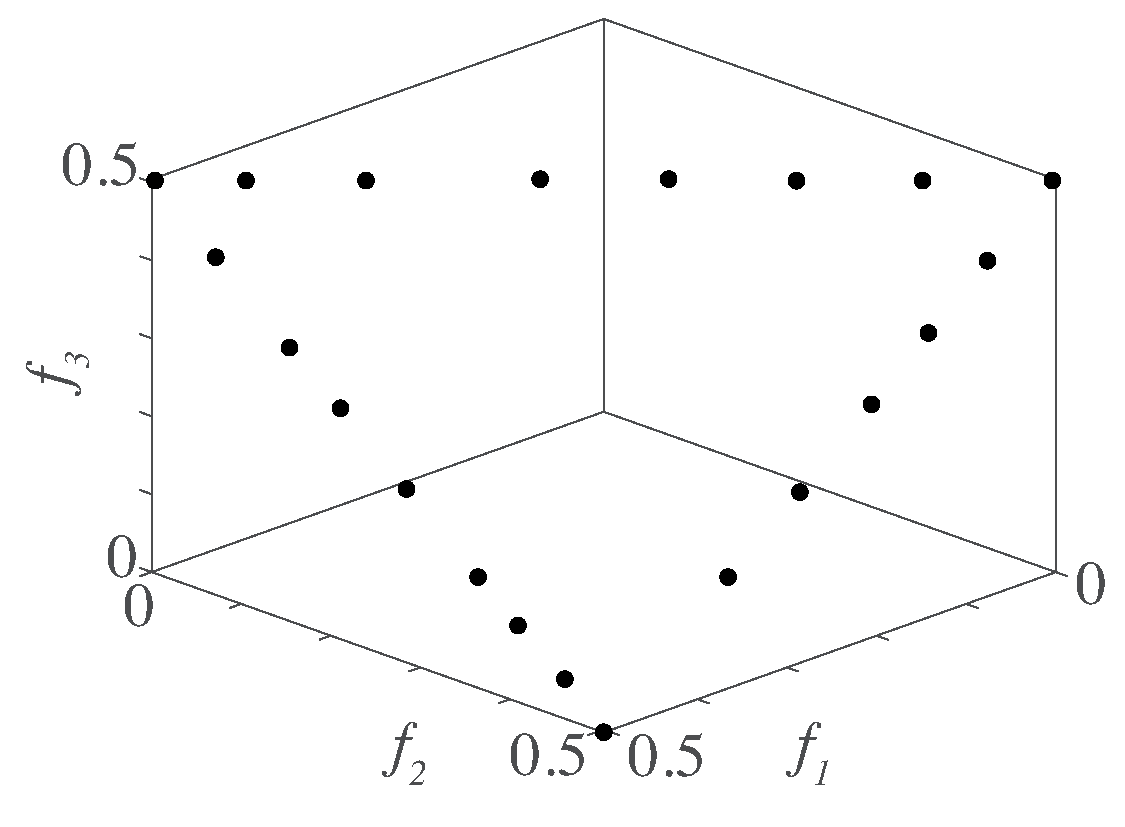
\includegraphics[width=1.5in]{FVEMOA_IDTLZ1_evaluation10000_r5_N21}}\\
  \caption{The final distribution of solutions set in the inverted-DTLZ1 problem.
  The algorithm is FV-EMOA with population size $=21$($H=5$) and evaluation number $=20000$.
  $r=1.2$ is the optimal setting and we observed a evenly distribution in (\ref{dm1:a}).
  As the increasing of $r$, solutions are more likely to be at the boundary
  (\ref{dm1:b}-\ref{dm1:d}). 
  }
  \label{dm1}
\end{figure}

For simply illustration, we only consider flat(not concave or convex) pareto front problem
in this paper.
When algorithm reach to the final stage, all solutions are near the pareto front, $r$ should
be specified as $1+1/H$, as in equation \ref{e1}. 

% ------------------sub-------------- dynamic mechanism ----------------------------------
% --------------- reference point specification for convergence ----------------
% hisao指出如果一直用1+1/H, 在convergence阶段会有不好的 search behavior,因为
% specify 1+1/H in each generation, 在 early generations
% the estimated ideal and nadir points from the nondominated
% solutions in each generation 离PF太远。
% 因此 对于normalization based on the estimated ideal and nadir points 
% often has unexpected bad effects on the search behavior
%
% in early generations, a slightly larger r is suggested in 【hisao和我的本科毕设】
% 大一点的r能够加快convergence 用NHV试试 log(HV)
% (加图 相同的evaluation 一直optimal和一直2 一直2会快点收敛 一个HV 一个NHV, 
% HV表示最后hv差,NHV表示较快到达前沿)
% (图 r越大,收敛越快,从三维开始 画出hv变化斜率图)
% 
\subsection{Reference Point Specification for Convergence}
However in the early stage, solutions set is not close to the pareto front, which makes the 
estimated ideal and nadir points far away from true ideal and nadir points, for the reason that
they are calculated by current nondominated solutions in each generation.
As a result, the search behavior will be poor for the poor normalization\cite{hisao, hisao26}.

In \cite{hisao}, a larger value of $r$ than the suggested value $1+1/H$ is used
in the early stage.

% ------------------sub-------------- dynamic mechanism ----------------------------------
% ------------------------- linearly decrease mechanism --------------------------
% so r从2到1+1/H 很必要 之前介绍过 但是怎么变化 没有一个特别好的idea outperform the others
% hisao的paper,提到一种linearly decrease 机制 就是从2到1+1/H线性下降 这是一种简单又实用的idea
% 图在下一个section画。
% 接下来本文介绍一种基于weak convergence detection criterion, 在一些限制条件下outperform线性机制。
% 
\subsection{Linearly Decrease Mechanism}
Based on the theory above, $r$ is suggested to be specified dynamically at different stages of
the algorithm(at early stage, a slightly larger $r$ is chosen; at final stage, $r=1+1/H$ is chosen).
But unfortunately, there is no best mechanism on how to specify value of $r$ dynamically
outperforms the others in all problems and all experiments settings. One mechanism may be the best
when work on some specific experiments conditions, but may be not good on other conditions. 

In \cite{hisao}, a linearly decrease mechanism has been proposed:
\begin{equation}\label{e2}
  r(t)=r_{Initial}\frac{(T-t)}{T}+(1+1/H)\frac{t}{T}, t=0,1,\dots,T,
\end{equation}
where $T$ is the total number of generations, and $r_{Initial}$ is the initial value of $r$,
which is larger than $1+1/H$.
It is a simple and practical mechanism. In (\ref{e2}), the value of $r$ starts from $r_{Initial}$,
then gradually decrease to the suggested value in a linearly decrease process. 
As shown in Fig. \ref{ldm1}.

In next section, we will propose another good dynamic mechanism based on weak convergence 
detection criterion outperform simple linearly decrease mechanism on some constraint condition.

% -------------------------------- new dynamic mechanism ------------------------------------
% 本文介绍一种基于weak convergence detection criterion的 new mechanism
% 当 检测到convergence 就把r从2变成optimal 
% (画 r 随 evaluation变化图 就是z字型那个 和线性机制一起画)
% 
\section{New Dynamic Mechanism}
In this section,
we will introduce a new mechanism that uses a weak convergence detection criterion to 
decide whether to change the value of $r$ from $r_{Initial}$ to $r_{Optimal}=1+1/H$. 

As we have explained before, 
a slightly larger $r$ is suggested at the initial stage of the algorithms. 
But for well diversity at the final stage,
it is needed to set $r$ to it's optimal value ($1+1/H$). 
For this purpose, we detect whether algorithm has convergenced or not. If solutions are all close to the 
pareto front, we change the value of $r$ to $r_{Optimal}$; otherwise, we set value of $r$ to 
$r_{Initial}$. The mechanism is also shown in Fig. \ref{ldm1}

% \begin{figure}[!t]
%   \centering
%   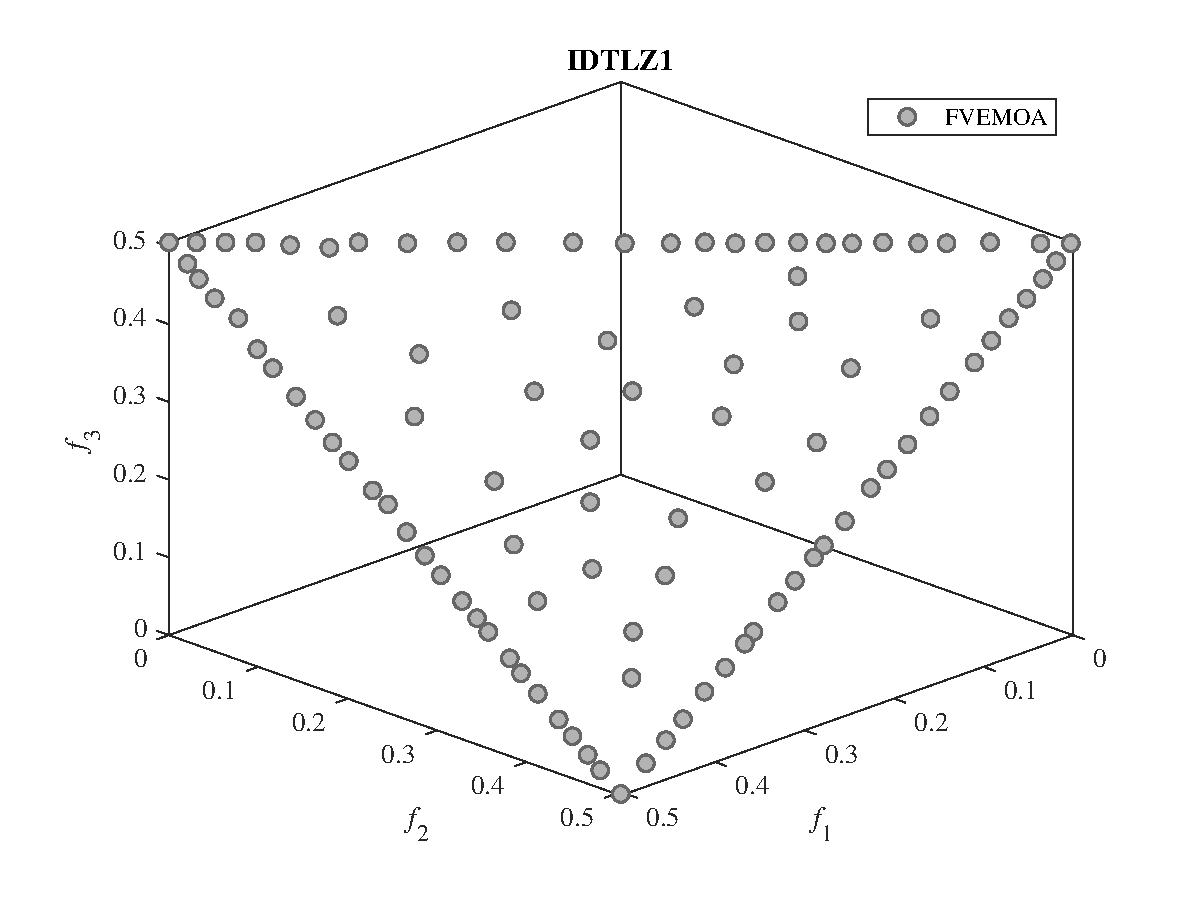
\includegraphics[width=\columnwidth]{FVEMOA_IDTLZ1}
%   \caption{}
%   \label{ldm1}
% \end{figure}

% ---------------sub-------------- new dynamic mechanism ------------------------------------
% ----------------------------- weak convergence detection ----------------------------------
% consider some convergence detection paper【各种 convergence detection paper】
% convergence detection一般用各种各样的indicator【各种paper】
% 总结特点:用indicator list的太花时间;精确的收敛检测
%
% 准则:
% convergence detection 不应该花太多时间,并不需要太准  用 subsubsection
% 需要寻找一种不需要花太多计算量的 weak criterion
% 【一些paper】indicator based algorithm用indicator
% for us,it seems to be a good idea to use HV 作为indicator,however
% 但是程序运行过程中 hv的reference point 一直在变,所以不同generations没有可比性
% (画一张算法运行过程中用的hv的图)
%
% estimated nadir point 会越来越接近PF, 并且当solutions reach to PF后 NaidrP stagnation
% (画 HV和bsf ln(nadir point) mean的图 最好用MaF1的 可能平滑些)表示它们同时期变化。 
% good idea to use ln(nadir point) mean作为判断解是否reach to PF 的 indicator
% 一篇论文(Introducing a Robust and Efficient Stopping Criterion for MOEAs)实现了
% the Least Squares Stopping Criterion for convergence detection 
% when indicator has reached a stagnation situation, stop
% 用一种简单并且直观SIMPLE INTUITIVE 的方式 就是剩余价值和线性回归斜率 below thresholds
% 介绍机制 线性计算公式
% 画上图(ln np mean)的b随evaluation变化图
% for nadir point, 经过我们的实验 10^-5是个好threshold
%
\subsection{Weak Convergence Detection}
Consider many convergence detection paper \cite{convergence detection},
various indicators including convergence detection indicators are using to detect the stagnation.
They focus on accuracy of convergence, which is not the purpose in our approach for 
the reason that after algorithm convergent, we still need some generations in order to
get evenly distribution of solutions set. 
We summarize our weak convergence detection criterions as follow:
\subsubsection{inaccuracy} It is no need to have a accurate convergence detection. 
The convergence can be reported if current solutions are close to the pareto front.
In other words, the estimated ideal and nadir points based on the current solutions
are close to the true ideal and nadir points. 
\subsubsection{saving time} We should not spend too much time in convergence detection
for the reason that the state-of-the-art indicator-based algorithms such as SMS-EMOA and HypE, 
are time consuming when dimension is very high. 

We are discussing the effect of reference points in calculating hypervolume. It seems to be a good
idea to use hypervolume as our convergence detection indicator, for that we have calculated
hypervolume in each generation in hypervolume-based evolutionary multi-objective optimization algorithm.
But during the process of algorithm, the reference point is calculated in (\ref{frpa1}) 
for each generation.
So we can not compare hypervolume among different generations. As shown in Fig. \ref{wcd1}
% \begin{figure}[!t]
%   \centering
%   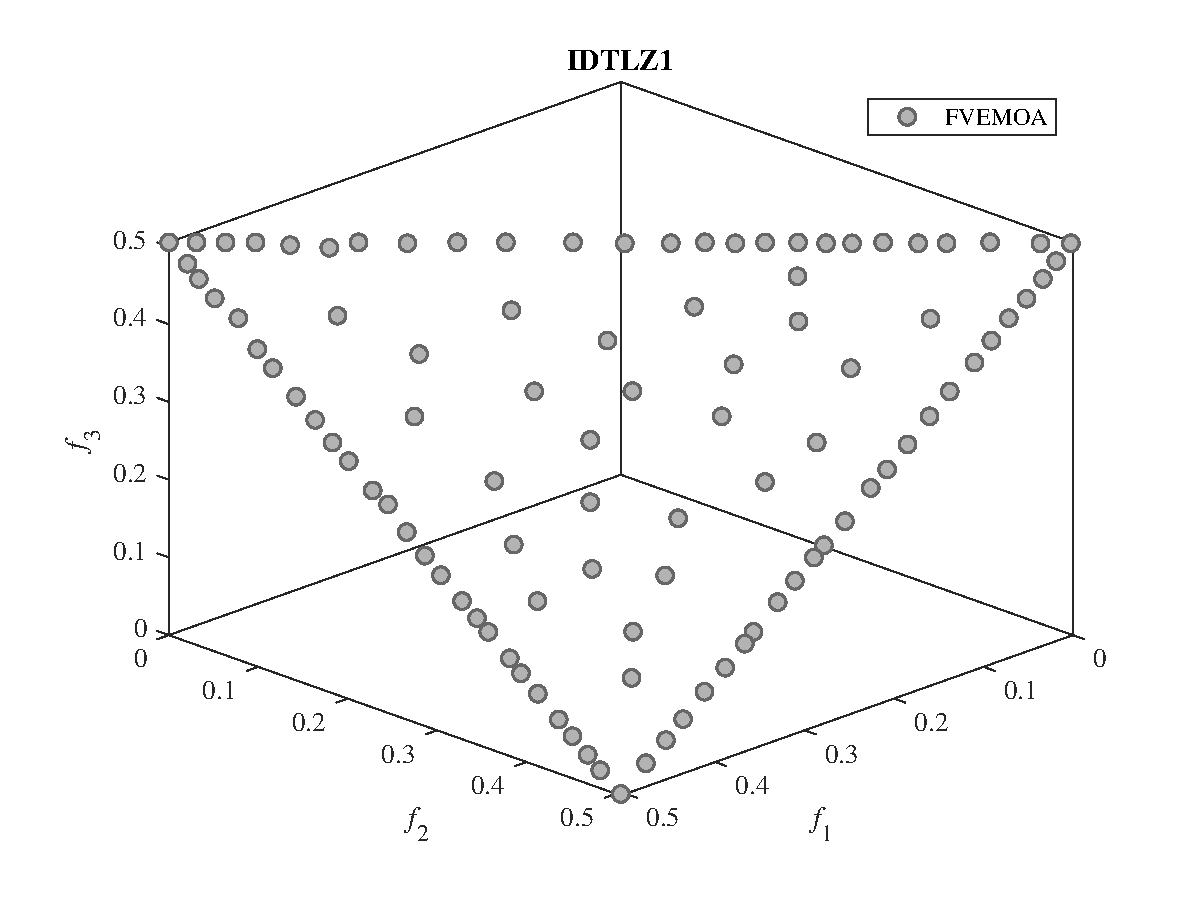
\includegraphics[width=\columnwidth]{FVEMOA_IDTLZ1}
%   \caption{}
%   \label{wcd1}
% \end{figure}

We are trying some other good indicators satisfying our convergence detection criterions. 
In Fig. \ref{wcd2} ,when current solutions are close to the pareto front, the estimated nadir point is close 
to the true nadir points. 
This imply that the estimated nadir point can be a good indicator for our purpose. 
But for some problems with large feasible region, 
the moving distance of estimated nadir point in the early generations is larger than that near convergence.
So we consider the logarithm. And consider the possible bad variance of the indicator, 
finally we use best logarithmic nadir point so far as our indicator. more specifically,
for a minimization problem, we consider the indicator as follows:
\begin{equation}\begin{aligned}\label{e3}
  ENP_{t} &= [f_{t1},f_{t2},\dots,f_{tm}]^\top \in \mathbb{R}^m ,\\
  I_{0} &= \frac{1}{m} \sum_{i=1}^{m}lnf_{0i},\\
  I_{t} &= min(I_{t-1},\frac{1}{m} \sum_{i=1}^{m}lnf_{ti}),
  t = 1,2,\dots,T,
\end{aligned}
\end{equation}
where $T$ is the total number of generations, 
$ENP_{t}$ is the estimated nadir point at the $t$th generation with $m$ objectives $f_{t1},f_{t2},\dots,f_{tm}$. 
$I_0$ is the initial indicator calculated by the initial population.
And $I_t$ is the minimum value before the $t$th generation (including the $t$th generation). 

After chosen the indicator, the next step is to detect the stagnation of indicator.
We use a basic linear regression method called Simple Least Squares\cite{lscd27} with a
simple least squares convergence detection strategy introduced in \cite{lscd}.
If the absolute value of slope of indicator is below a threshold, the convergence is reported.
Briefly speaking, the intercept $a$ and slope $b$ of the $t$th generation can be calculated 
with the following matrix-based formula:
\begin{equation}\label{e4}
  \left[
    \begin{matrix}
      a \\
      b
    \end{matrix}
  \right]
  = 
  \left[
    \begin{matrix}
      \sum t_i^2 & \sum t_i \\
      \sum t_i   & w\_ l 
    \end{matrix}
  \right]^{-1}
  *
  \left[
    \begin{matrix}
      \sum t_i * I_{t_i} \\
      \sum I_{t_i} 
    \end{matrix}
  \right]
\end{equation}
where $w\_ l$ is the length of the chosen window 
and $t_i$ is the generation number in the chosen window.
The value of slope $b$ is shown in Fig. \ref{wcd2} 
(Note that the value in the first $w\_ l$ generations is 0, 
and we should not consider the first $w\_ l$ generations). 

With the above formula (\ref{e4}), the convergence detection criterion is defined as:
\begin{equation}\label{e5}
  convergence = \vert b \vert < thres
\end{equation}
The chosen of the $thres$ value is not so important 
as the report ahead or delay is not fatal to the algorithm or to the final solutions set.
We choose the $thres$ value as $10^{-5}$ after some experimental computation with 
the window size $w\_ l = 100$. 
If we do not change the window size, 
this threshold can be applied to other problems or indicator-based algorithms
because of a weak convergence detection purpose.

% \begin{figure}[!t]
%   \centering
%   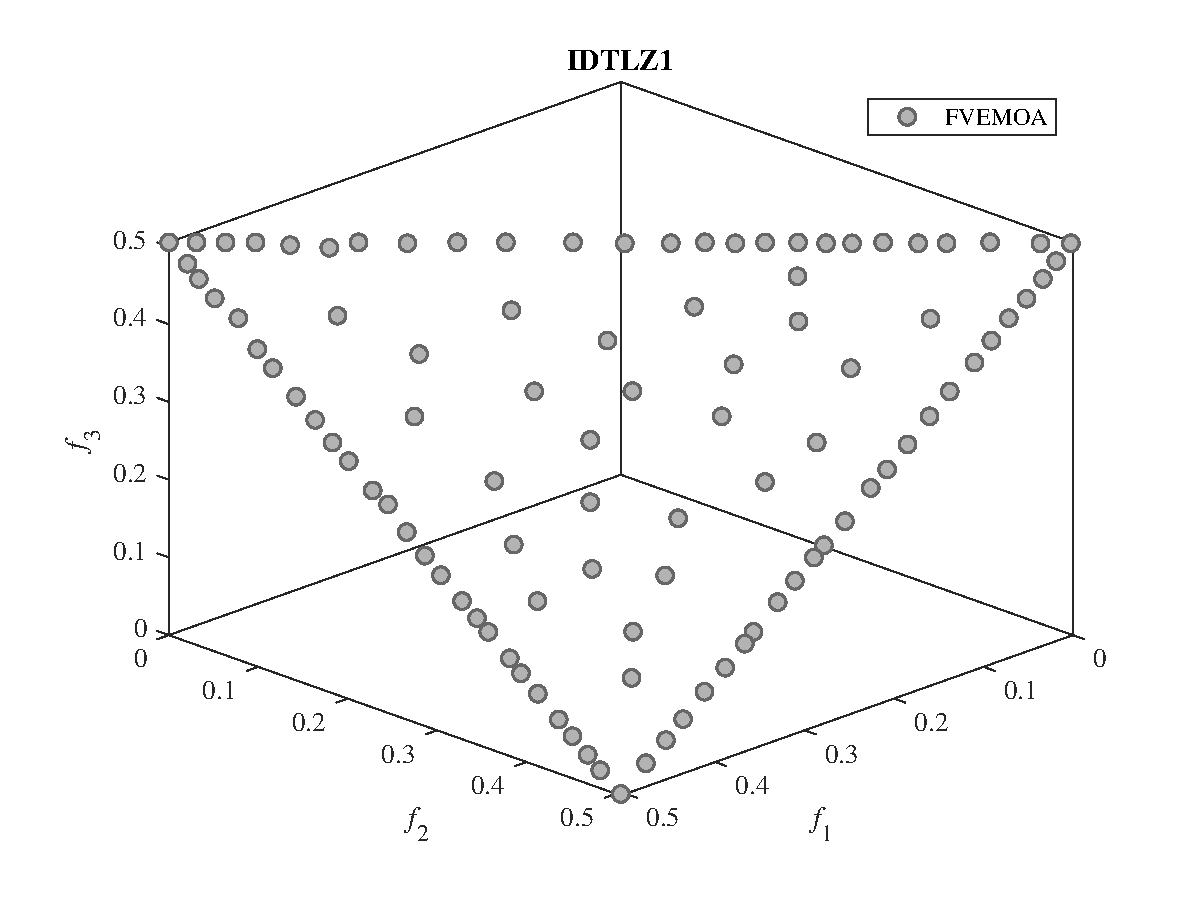
\includegraphics[width=\columnwidth]{FVEMOA_IDTLZ1}
%   \caption{}
%   \label{wcd2}
% \end{figure}

% -------------------------------- Computational Experiments ------------------------------------
% 为了直观的表现dynamic reference point adaptation的优势,
% 算法 sets 我们选用了什么,简单介绍
% 我们选用了test problem:DTLZ1, C1_DTLZ1,IDTLZ1,MaF1 分别介绍
% 维度选择了 3,5,8,10维 为了表现在multi 和 many上的不同
% 
% compare this mechanism with the linearly decrease mechanism
% 
% 要验证 10^-5 是不是一个好的threshold 画出不同维度 当检测到收敛的solutions图,确认检测到不变的时候确实收敛
%
\section{Computational Experiments}

\subsection{Settings}

\subsection{Computational Results}

% ---------------sub-------------- Computational Experiments ------------------------------------
% ----------------------------- comparison of two dynamic mechanism ----------------------------------
% 2种机制比较
% 当evaluation足够的时候,差不多
%
\subsection{Comparison of Two Dynamic Mechanism}


\section{Conclusion}
The conclusion goes here.


% use section* for acknowledgment
\section*{Acknowledgment}


The authors would like to thank...\cite{IEEEhowto:kopka1}





% trigger a \newpage just before the given reference
% number - used to balance the columns on the last page
% adjust value as needed - may need to be readjusted if
% the document is modified later
%\IEEEtriggeratref{8}
% The "triggered" command can be changed if desired:
%\IEEEtriggercmd{\enlargethispage{-5in}}

% references section

% can use a bibliography generated by BibTeX as a .bbl file
% BibTeX documentation can be easily obtained at:
% http://www.ctan.org/tex-archive/biblio/bibtex/contrib/doc/
% The IEEEtran BibTeX style support page is at:
% http://www.michaelshell.org/tex/ieeetran/bibtex/
%\bibliographystyle{IEEEtran}
% argument is your BibTeX string definitions and bibliography database(s)
%\bibliography{IEEEabrv,../bib/paper}
%
% <OR> manually copy in the resultant .bbl file
% set second argument of \begin to the number of references
% (used to reserve space for the reference number labels box)
\begin{thebibliography}{1}

\bibitem{IEEEhowto:kopka}
H.~Kopka and P.~W. Daly, \emph{A Guide to \LaTeX}, 3rd~ed.\hskip 1em plus
  0.5em minus 0.4em\relax Harlow, England: Addison-Wesley, 1999.

\bibitem{IEEEhowto:kopka1}
H.~pka and P.~W. Daly, \emph{A Guito \LaTeX}, 3rd~ed.\hskip 1em plus
  0.5em minus 0.4em\relax Harlow, England: Addison-Wesley, 1999.

\end{thebibliography}




% that's all folks
\end{document}


